%!TEX root = ttc14-fixml.tex

\section{M2T Transformation Class Hierarchy}
\label{sec:M2TClassHierarchy}

\begin{figure}[h!bt]
  \centering
  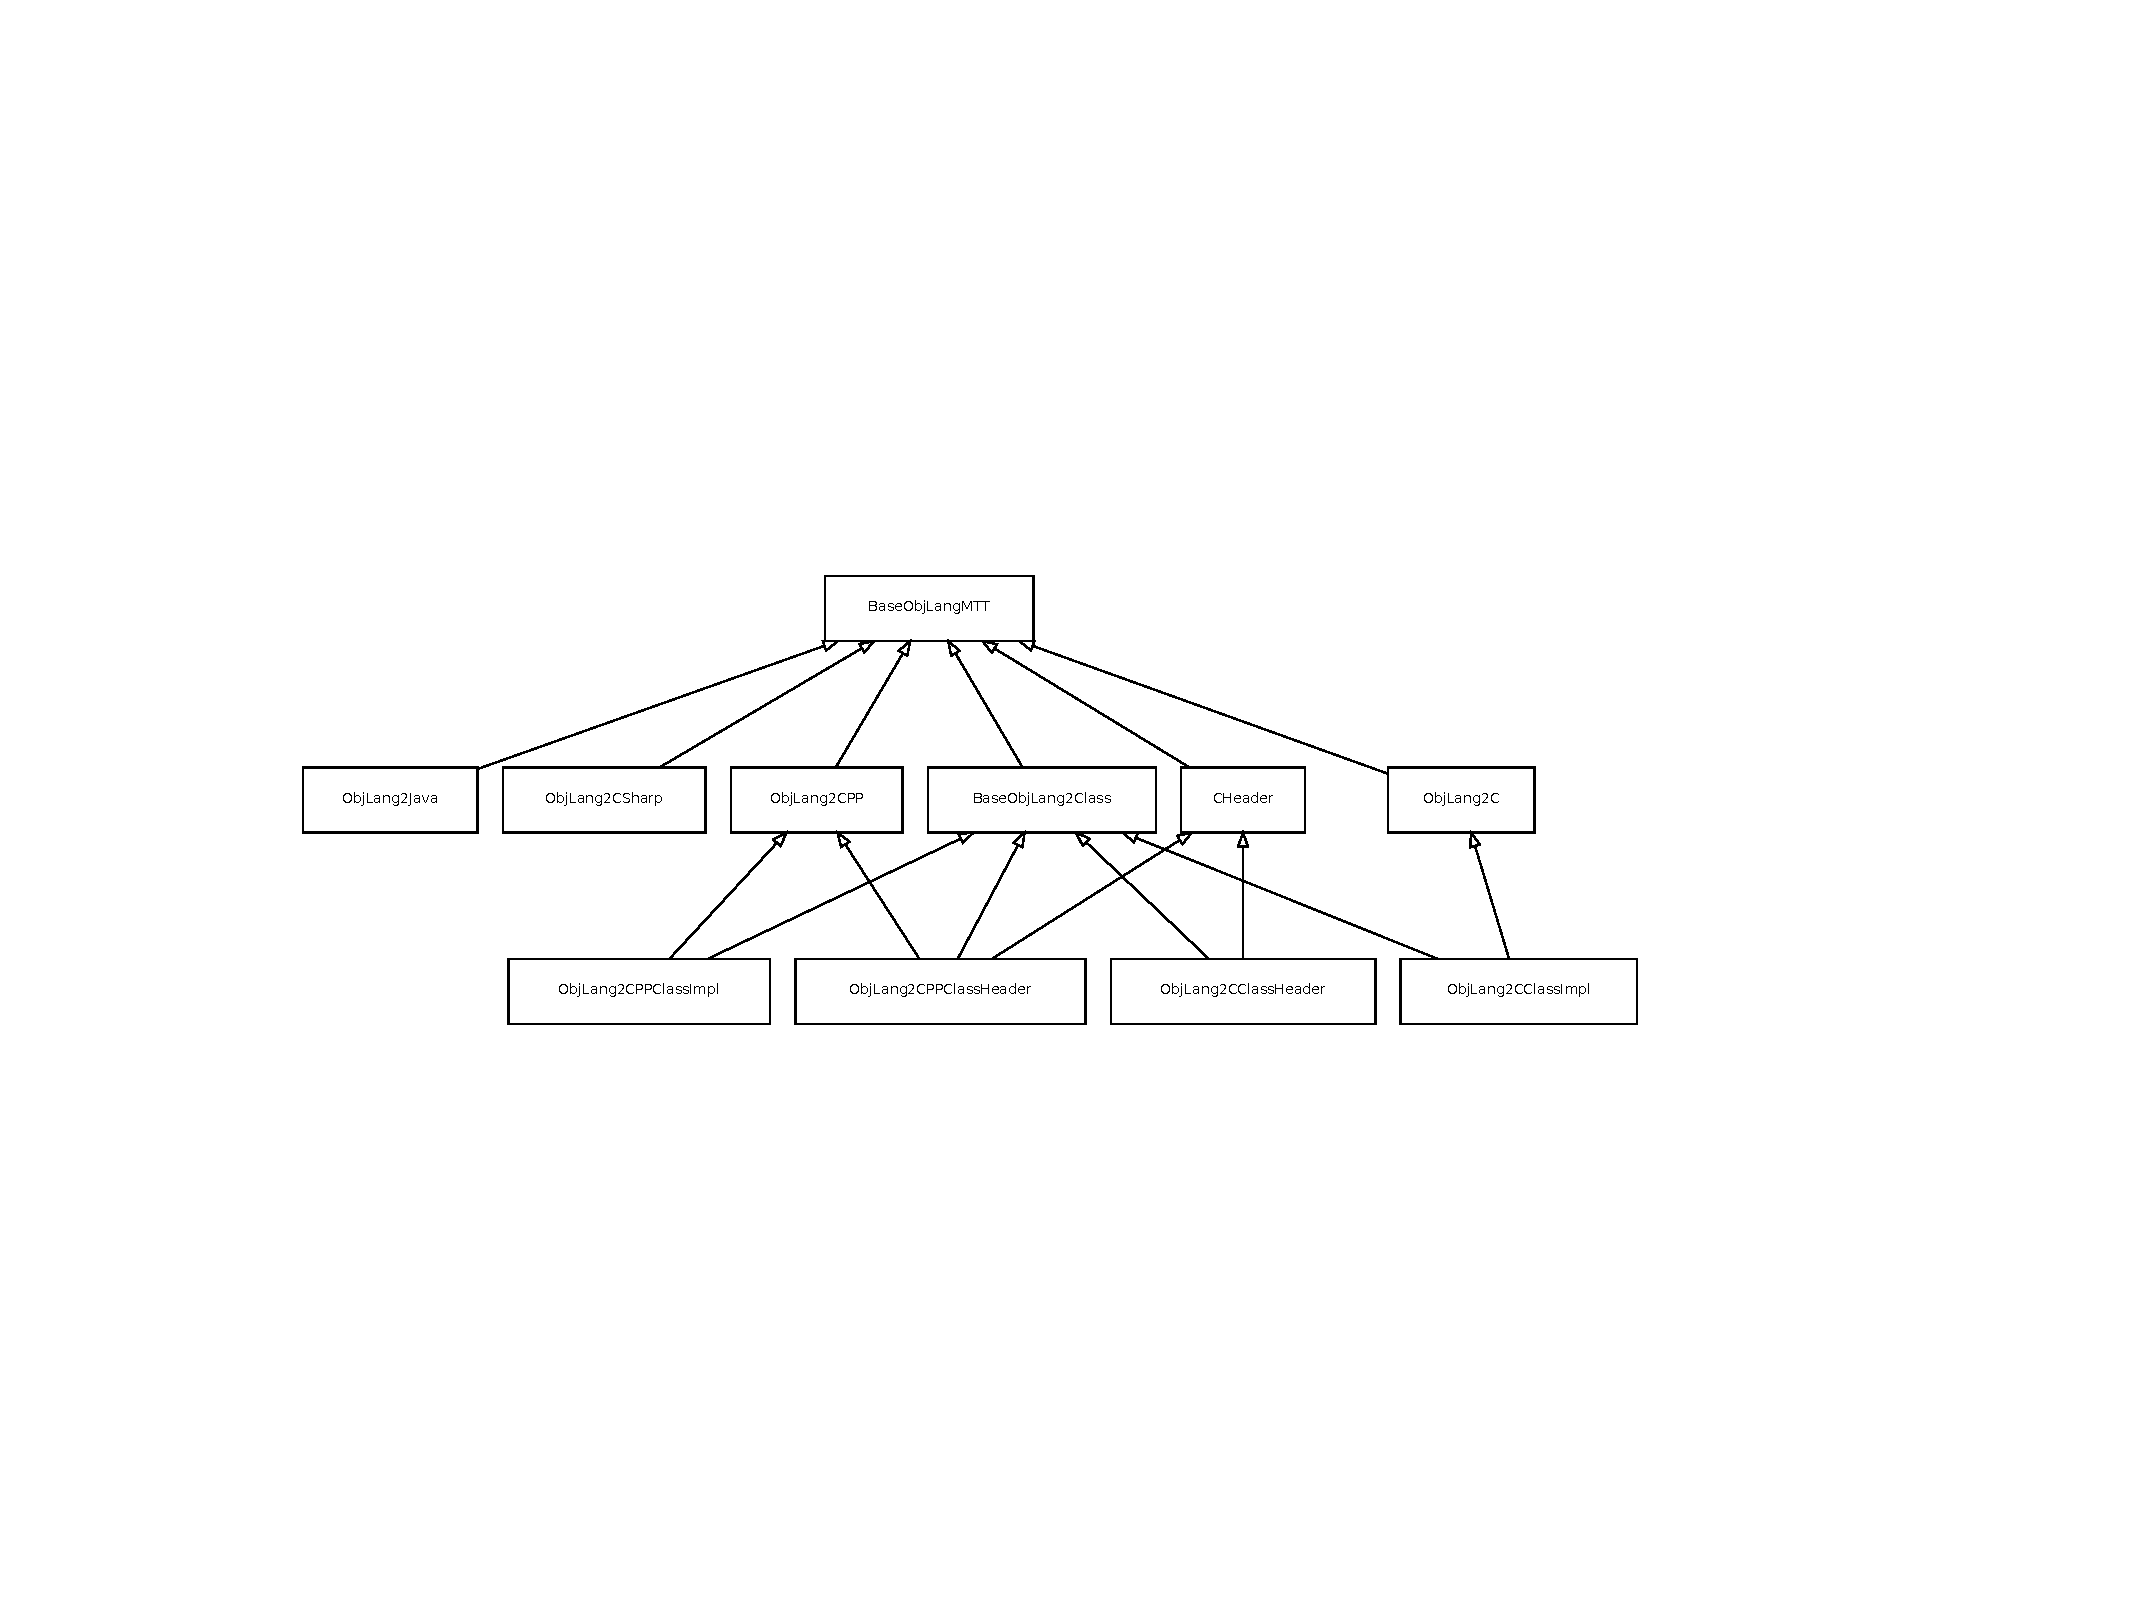
\includegraphics[width=\textwidth]{figures/M2TClassHierarchy.pdf}
  \caption{M2T transformation class hierarchy including C code generation}
  \label{fig:M2TClassHierarchy}
\end{figure}

\begin{table}
	\centering
  \begin{tabular}{l|l}
  \hline
  \textbf{File name}                  & \textbf{Source line of code} \\ \hline
  ObjLang2C.scala              & 50                  \\
  ObjLang2CClassImpl.scala     & 42                  \\
  ObjLang2CPPClassHeader.scala & 38                  \\
  BaseObjLangMTT.scala         & 35                  \\
  ObjLang2CClassHeader.scala   & 35                  \\
  BaseObjLang2Class.scala      & 33                  \\
  ObjLang2CPP.scala            & 27                  \\
  ObjLang2CPPClassImpl.scala   & 26                  \\
  ObjLang2Java.scala           & 15                  \\
  ObjLang2CSharp.scala         & 15                  \\
  CHeader.scala                & 15                  \\ \hline
  \textbf{Total}                        & \textbf{331}                 \\ \hline
  \end{tabular}
  \caption{Source lines of code for the complete M2T transformation including C code generation}
\end{table}